\paragraph{Average versus occurrence}\mbox{}\\
Another interesting analysis can be the study of the relation between the occurrence and the average expression. In figure~\ref{fig:scalinglaws/gtex/meanDiff_binned_sampling} it is shown the result, it is clear that there is a relation between occurrence and average, genes that express in more realizations (higher occurrence and right in the figure) have a higher average. Moreover, it doesn't exist genes that have high expression in few realizations; genes that are rare are also difficult to find so have a small average. Note that the average has got a bound due to the fact that counts are integer numbers, so if, for example, one gene express in $n$ of the $R$ samples, it has occurrence $O_i=\frac{n}{R}$ and its average can't be lower than $\avg{\mathrm{counts}}=\frac{1*n}{R}$
\begin{figure}[htb!]
    \centering
    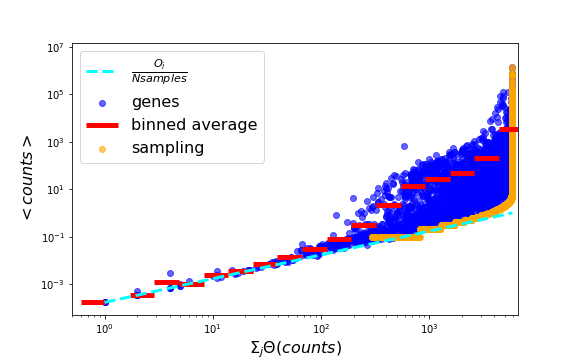
\includegraphics[width=0.9\linewidth]{pictures/scalinglaws/gtex/meanDiff_binned_sampling.png}
    \caption{Relation between the occurrence of a gene and its average across realizations.}
    \label{fig:scalinglaws/gtex/meanDiff_binned_sampling}
\end{figure}
